\documentclass[aspectratio=169]{beamer}
\usepackage[utf8]{inputenc}
\usepackage{hyperref}
\usepackage{amsmath,amsfonts,amsthm,bm}
\usepackage{color}
\usepackage{minted}
\usepackage{graphicx} % Allows including images
\usepackage{booktabs} % Allows the use of \toprule, \midrule and \bottomrule in tables
\usepackage{tikz}
\usepackage[version=3]{mhchem}
\usepackage{pgfplots}
\pgfplotsset{compat=1.16} 
\setminted{fontsize=\scriptsize}


\hypersetup{
    colorlinks=true,
    linkcolor=red,
    filecolor=magenta,      
    urlcolor=red,
}

\DeclareMathOperator*{\argmax}{argmax}
\DeclareMathOperator*{\argmin}{argmin}
\let \vec \mathbf

\newcommand{\classname}{NANOx81}
\newcommand{\classyear}{Fall 2022}
\mode<presentation> {
    \usetheme{CambridgeUS}
    \setbeamertemplate{footline}[text line]{%
      \parbox{\linewidth}{\vspace*{-8pt}\classname\hfill\classyear\hfill\insertpagenumber}}

    %\setbeamertemplate{footline}[page number]
    \setbeamertemplate{navigation symbols}{}
}


\title[Introduction to Data Science in Materials Science]{Introduction to Data Science in Materials Science}

\author{Shyue Ping Ong}
\institute[UCSD]{University of California, San Diego\\
\medskip
}
\date{\classyear} % Date, can be changed to a custom date

\begin{document}


\begin{frame}
    \titlepage % Print the title page as the first slide
\end{frame}


% \begin{frame}{Overview}
%     \tableofcontents
% \end{frame}


% \section{What is Data Science?}

\begin{frame}{What is Data Science?}
    \Huge{Data science is a multi-disciplinary field that uses scientific methods, processes, algorithms and systems to \textcolor{red}{extract knowledge and insights from structured and unstructured data}.}
\end{frame}


\begin{frame}{What is Data Science?}
    \begin{figure}
        \centering
        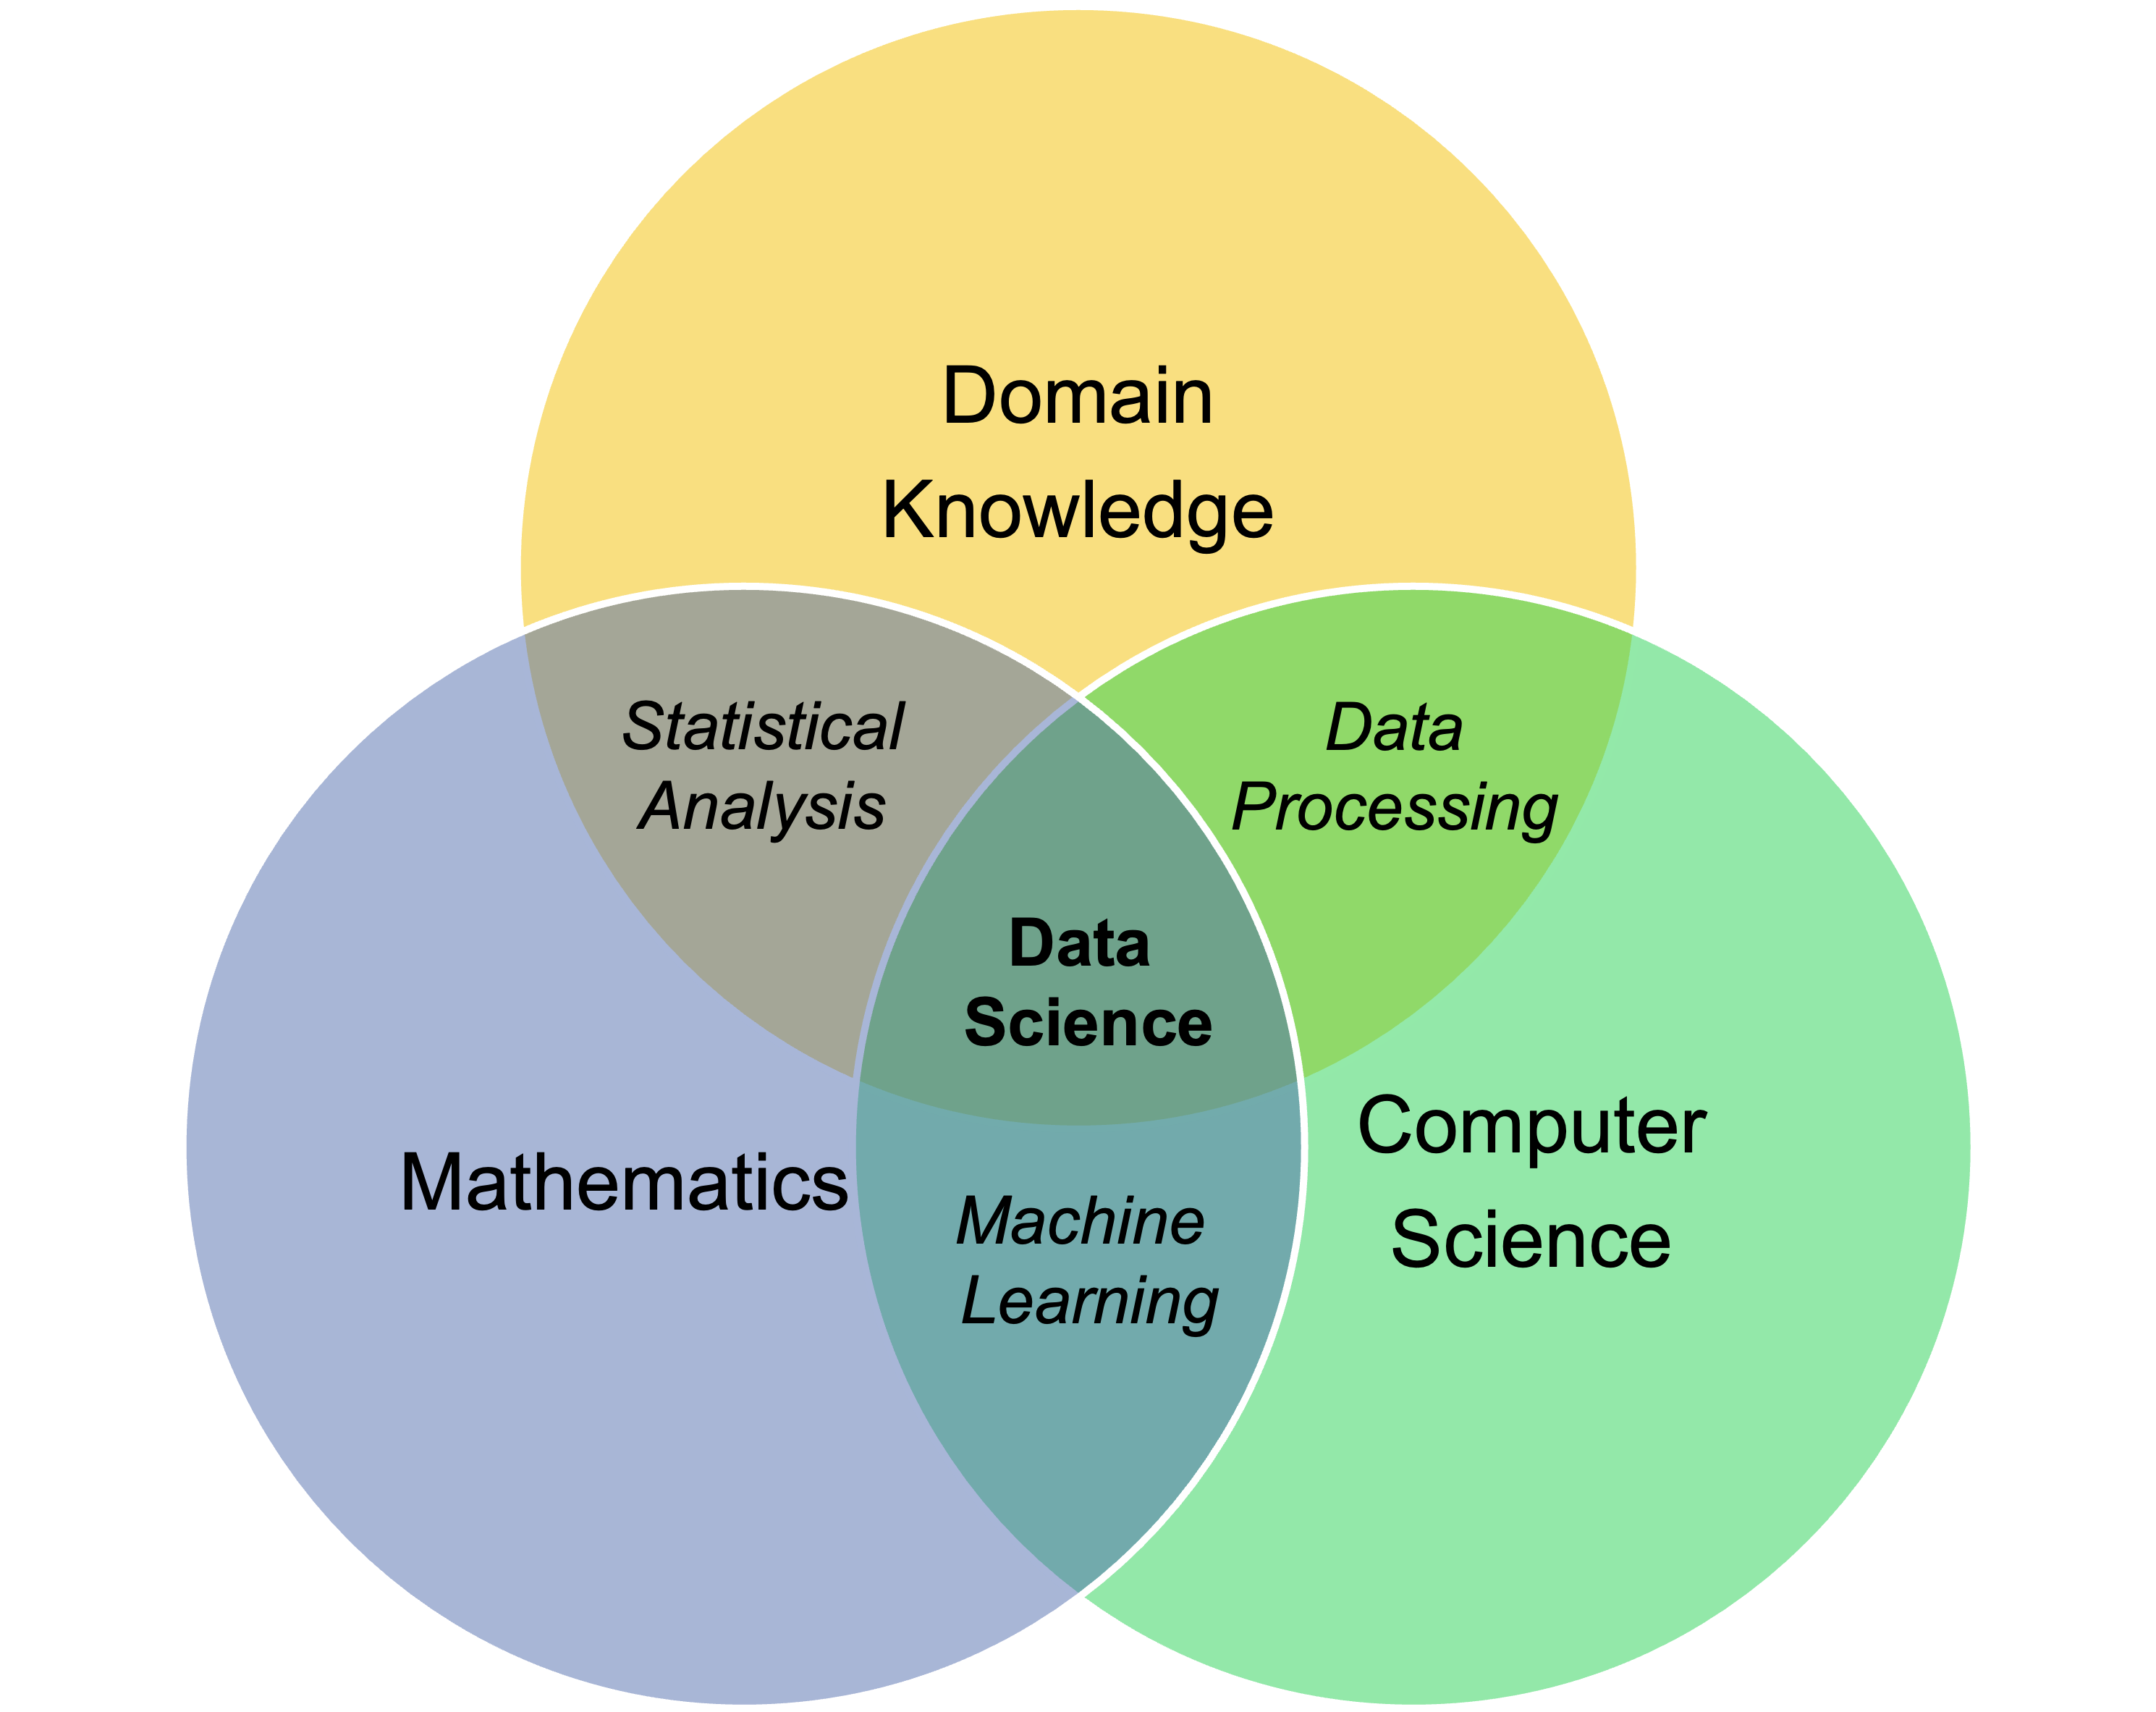
\includegraphics[width=0.5\textwidth]{lectures/slides_tex/datascience.png}    \end{figure}
\end{frame}

\begin{frame}{The Data Age}
    \begin{figure}
        \centering
        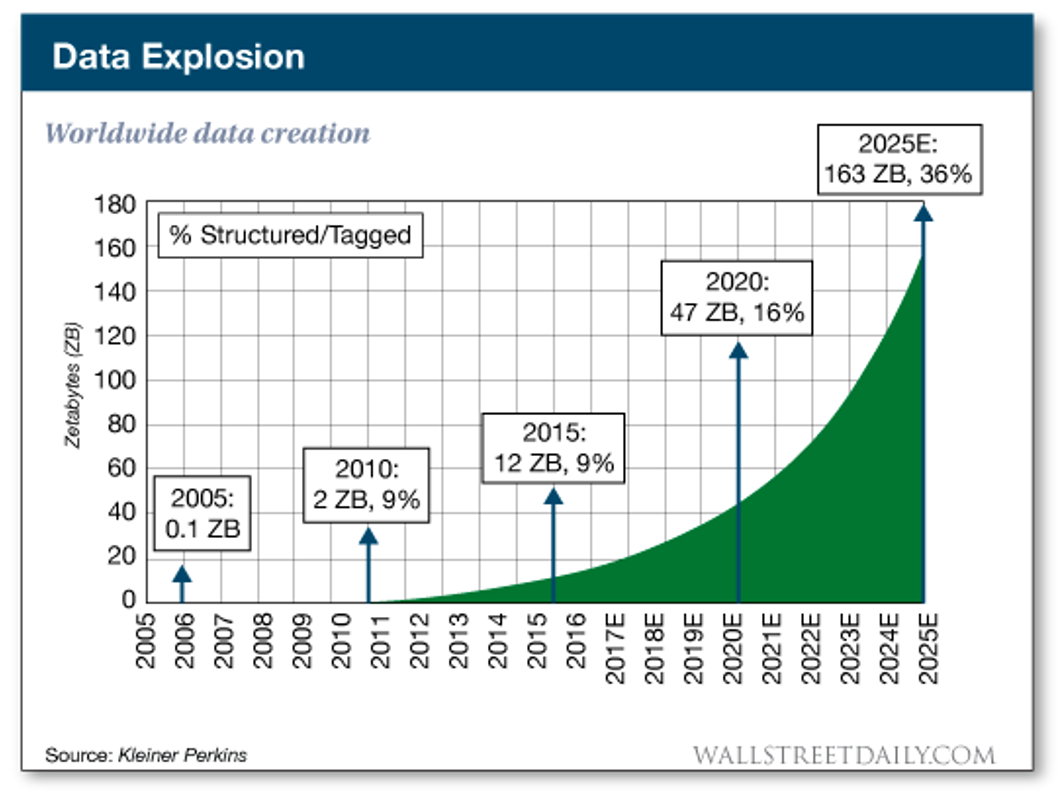
\includegraphics[width=0.6\textwidth]{lectures/slides_tex/worldwidedatacreation.png}
    \end{figure}
\end{frame}

\begin{frame}{Growth of Materials Data (as of Jan 1 2020)}

\begin{columns}
\column{0.5\textwidth}
\begin{figure}
        \centering
        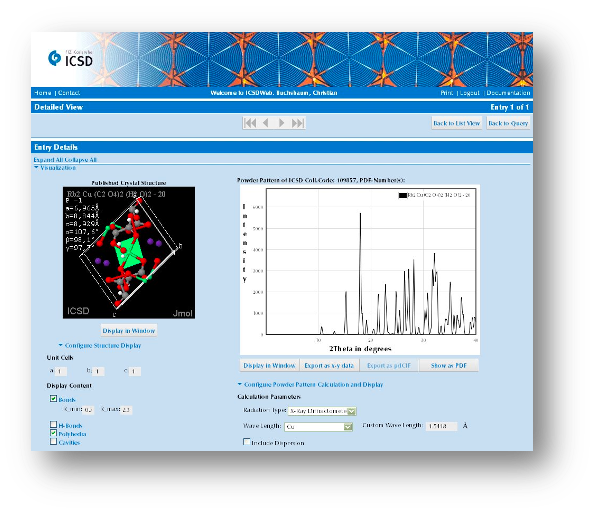
\includegraphics[width=0.4\textwidth]{lectures/slides_tex/icsd.png}
        \caption{ICSD: $\sim$200,000 crystals
}
    \end{figure}
    \begin{figure}
    \centering
    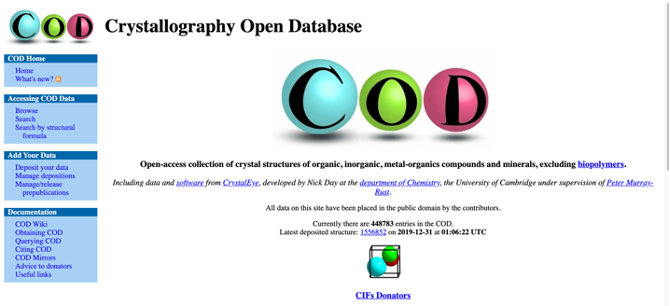
\includegraphics[width=0.4\textwidth]{lectures/slides_tex/cod.png}
    \caption{COD: $\sim$400,000 crystals
}
\end{figure}

\column{0.5\textwidth}
    \begin{figure}
        \centering
        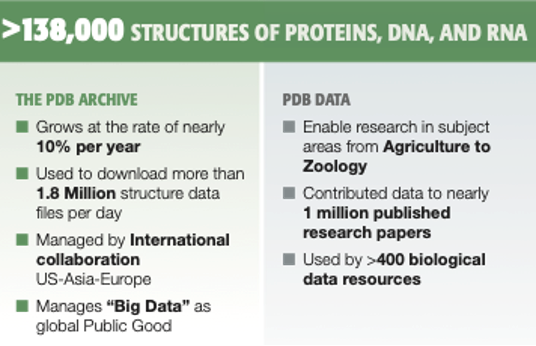
\includegraphics[width=0.4\textwidth]{lectures/slides_tex/pdb.png}
        \caption{Protein data bank}
    \end{figure}
\begin{figure}
    \centering
    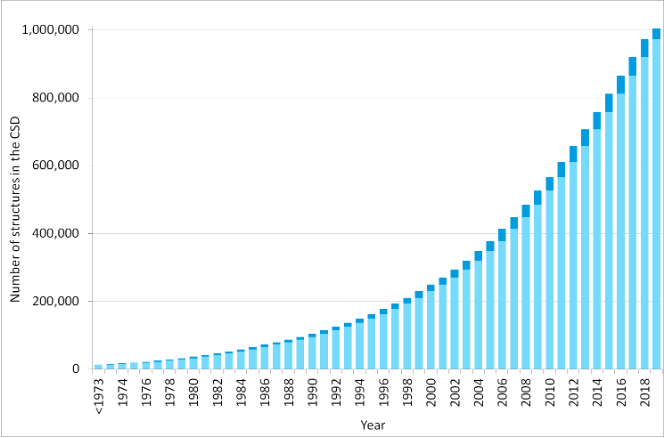
\includegraphics[width=0.4\textwidth]{lectures/slides_tex/csd.png}
    \caption{Cambridge structural database (small-molecule organic crystal structures)}
\end{figure}
\end{columns}
\end{frame}


\begin{frame}{But Quantity and Quality Lags Many Other Fields}

\begin{columns}
\column{0.5\textwidth}
\begin{figure}
        \centering
        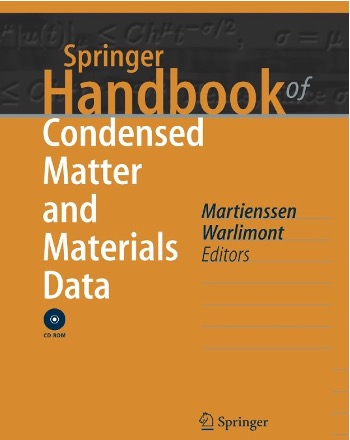
\includegraphics[width=0.45\textwidth]{lectures/slides_tex/handbook_of_condensed_matter.jpg}
        \caption{One of the most comprehensive handbooks on materials data: Density, thermal and electrical conductivity, melting and boiling points, etc., but O(100) binaries and limited ternaries...
}
    \end{figure}
\column{0.5\textwidth}
    \begin{figure}
        \centering
        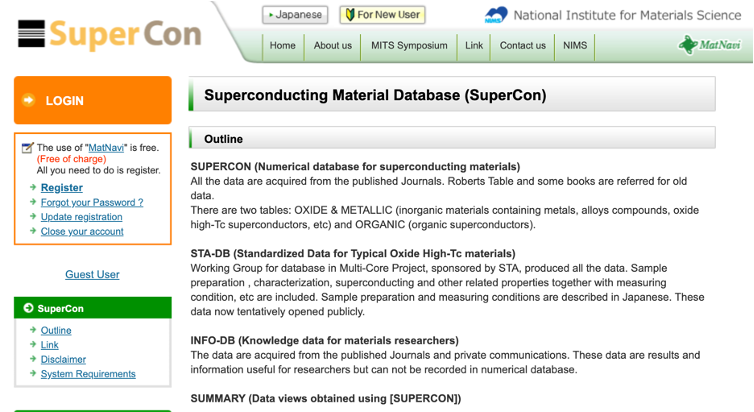
\includegraphics[width=0.9\textwidth]{lectures/slides_tex/supercon.png}
        \caption{$\sim$1000+ superconductors (many minor composition modifications). Ref: \url{ https://supercon.nims.go.jp/}
}
\end{figure}
\end{columns}
\end{frame}

\begin{frame}{First Principles Materials Computations}
    \begin{figure}
        \centering
        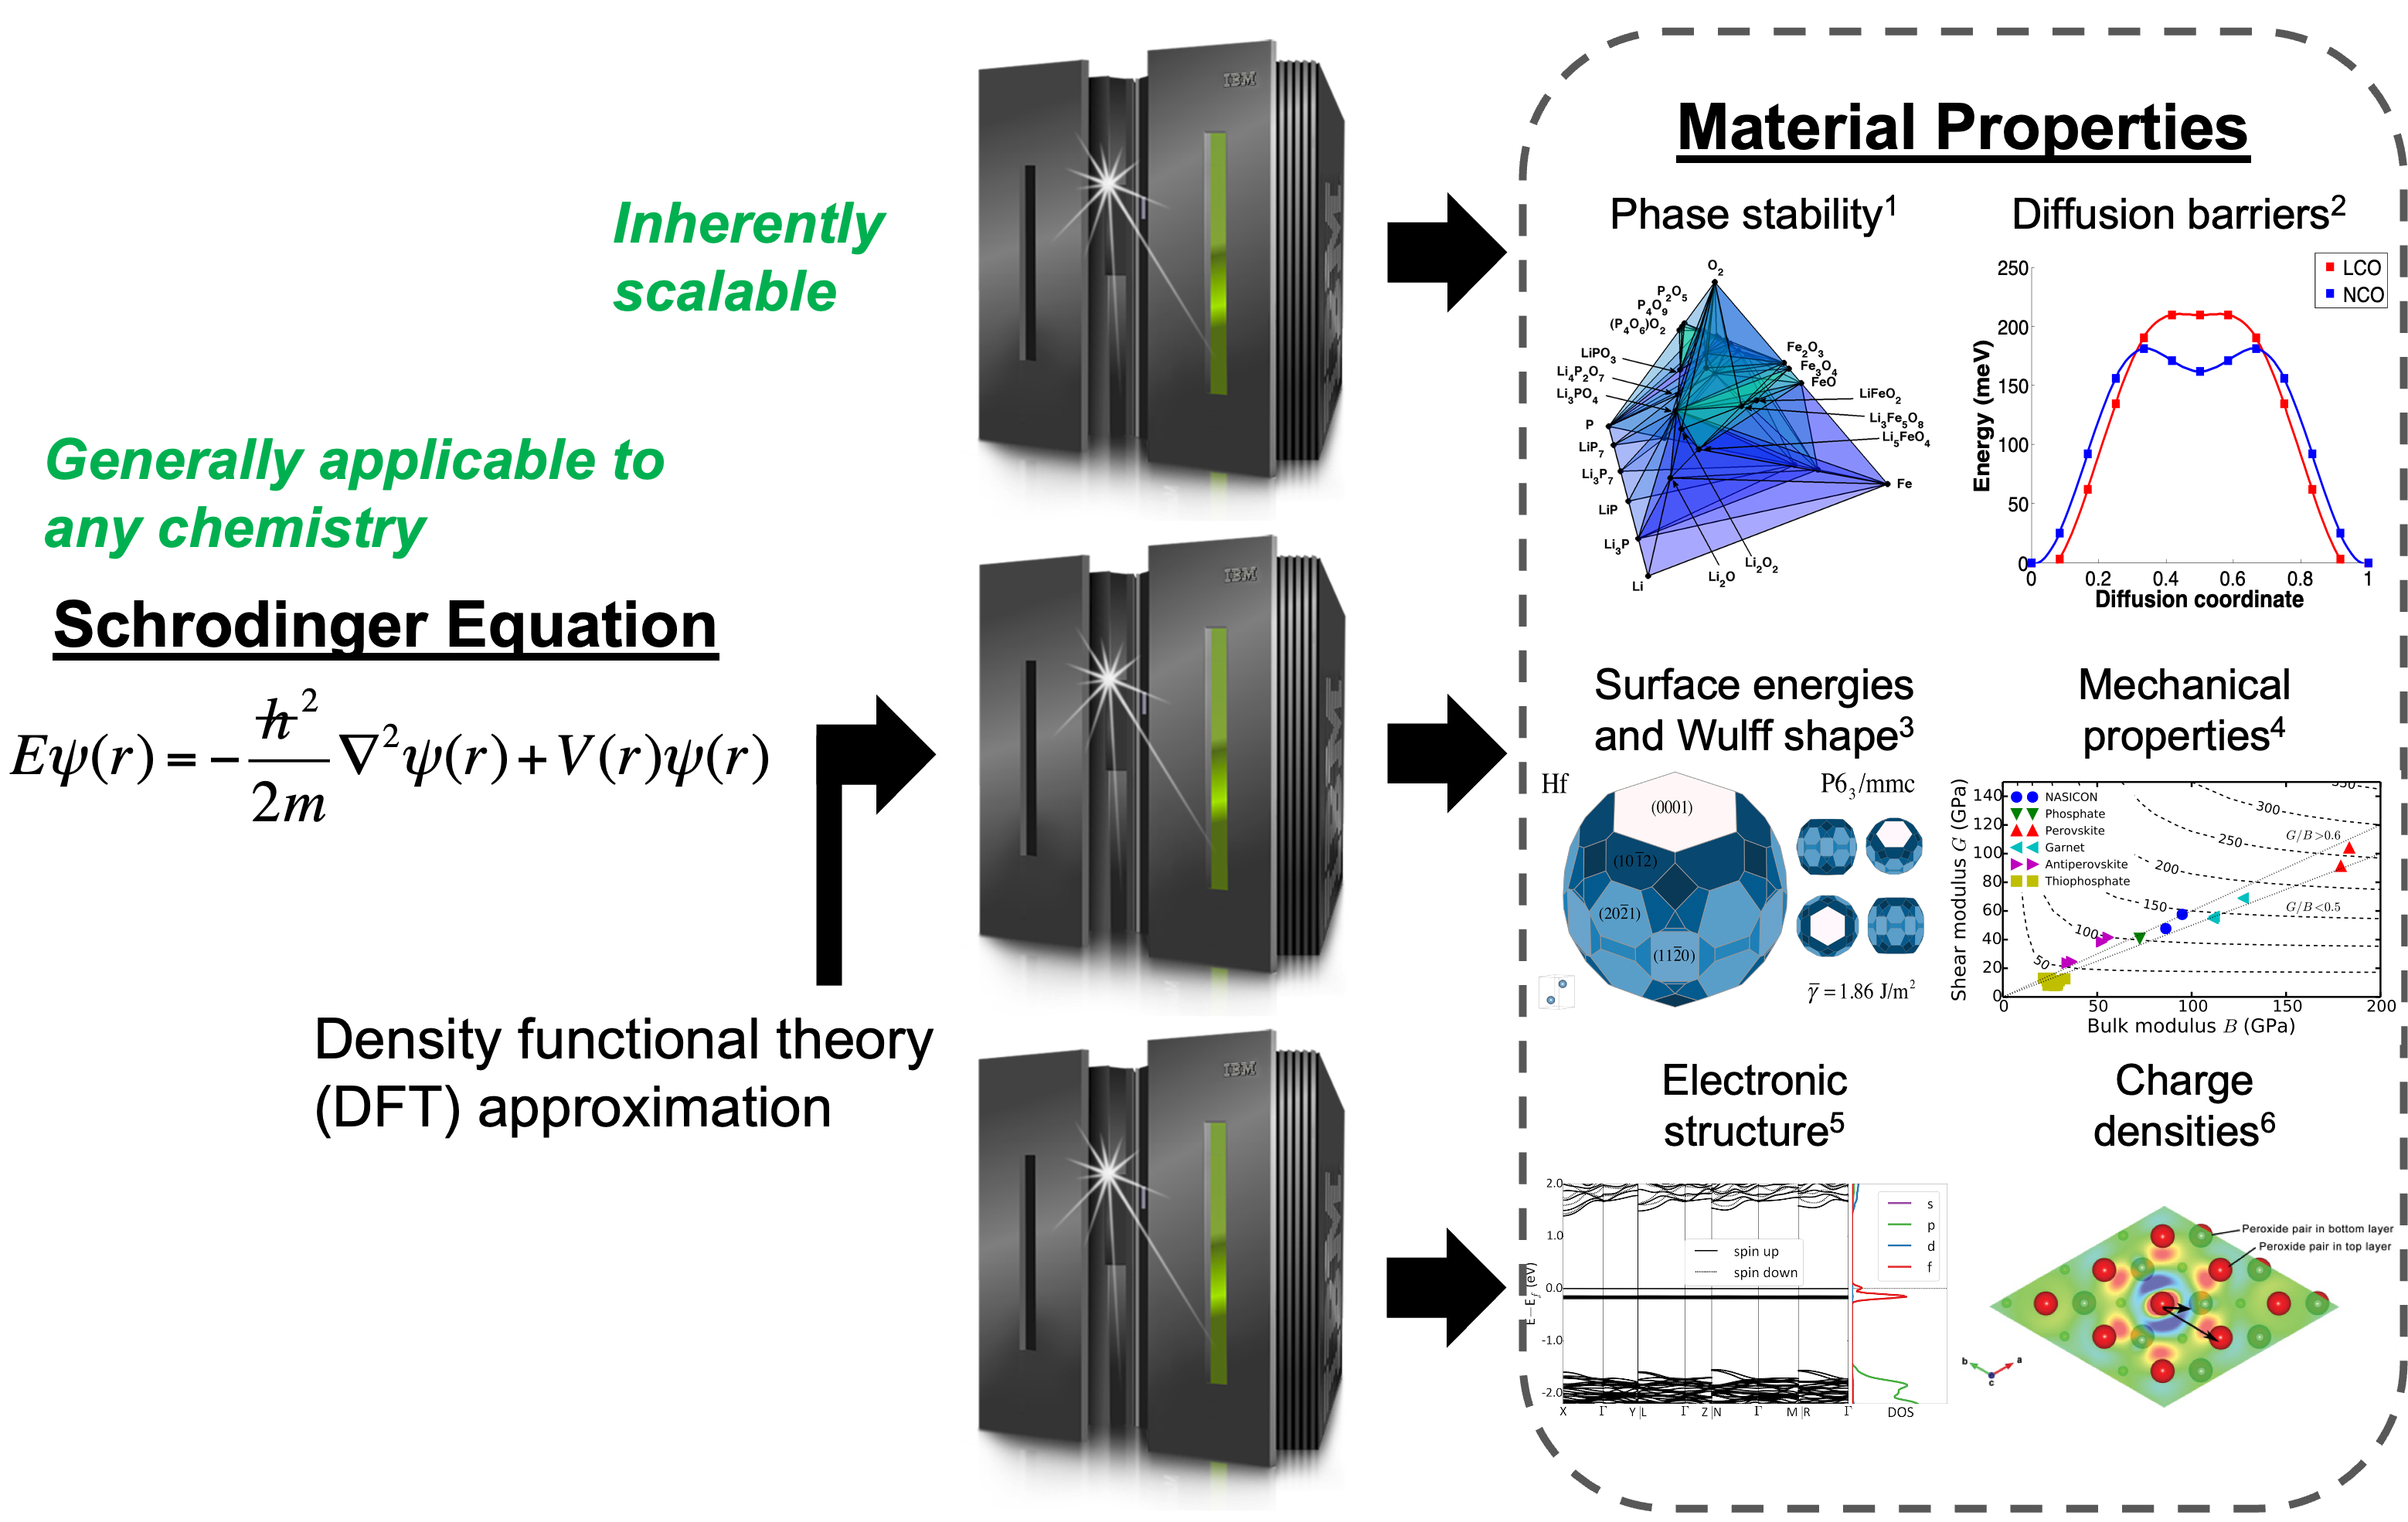
\includegraphics[width=0.7\textwidth]{lectures/slides_tex/computational_materials_science.png}
    \end{figure}
\end{frame}

\begin{frame}{Electronic structure calculations are today \textit{reliable} and \textit{reasonably accurate}...}

\begin{columns}
\column{0.2\textwidth}
\begin{figure}
        \centering
        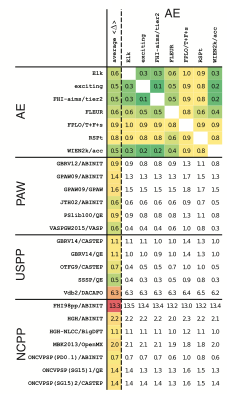
\includegraphics[width=\textwidth]{lectures/slides_tex/reliability_of_dft.png}
    \end{figure}
\column{0.5\textwidth}
    \begin{figure}
        \centering
        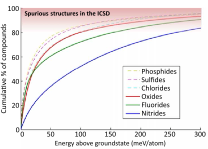
\includegraphics[width=0.45\textwidth]{lectures/slides_tex/icsd_e_hull.png}
        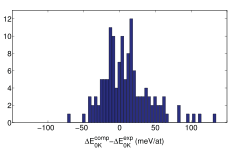
\includegraphics[width=0.45\textwidth]{lectures/slides_tex/formation_energies.png}\\
        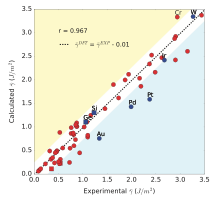
\includegraphics[width=0.45\textwidth]{lectures/slides_tex/surface_energies.png}
        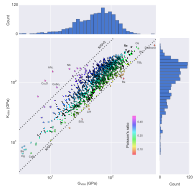
\includegraphics[width=0.45\textwidth]{lectures/slides_tex/elastic_constants.png}
\end{figure}
\column{0.2\textwidth}
\begin{itemize}
    \tiny
    \item (left) Modern electronic structure codes give relatively consistent equations of state.
    \item (right, clockwise from top left) Good predictions can be obtained for phase stability,\cite{sunThermodynamicScaleInorganic2016} formation energies, surface energies,\cite{tranSurfaceEnergiesElemental2016} and elastic constants\cite{dejongChartingCompleteElastic2015}.
\end{itemize}
\end{columns}
\end{frame}

\begin{frame}{Software frameworks for high-throughput computational materials science}
\begin{itemize}
    \item Materials Project (\url{https://materialsproject.org})\cite{jainCommentaryMaterialsProject2013}
    \begin{itemize}
        \item Python Materials Genomics or pymatgen (\url{https://pymatgen.org})\cite{ongPythonMaterialsGenomics2013}
        \item Custodian (\url{https://materialsproject.github.io/custodian/})
        \item FireWorks \cite{jainFireWorksDynamicWorkflow2015}
    \end{itemize}
    \item Atomic Simulation Environment (\url{https://wiki.fysik.dtu.dk/ase})
    \item AFLOW (\url{http://aflowlib.org})\cite{curtaroloAFLOWLIBORGDistributed2012}
    \item AiiDa (\url{http://www.aiida.net})
\end{itemize}
\end{frame}


\begin{frame}{Computation + Automation $\rightarrow$ Large databases}
\begin{figure}
    \centering
    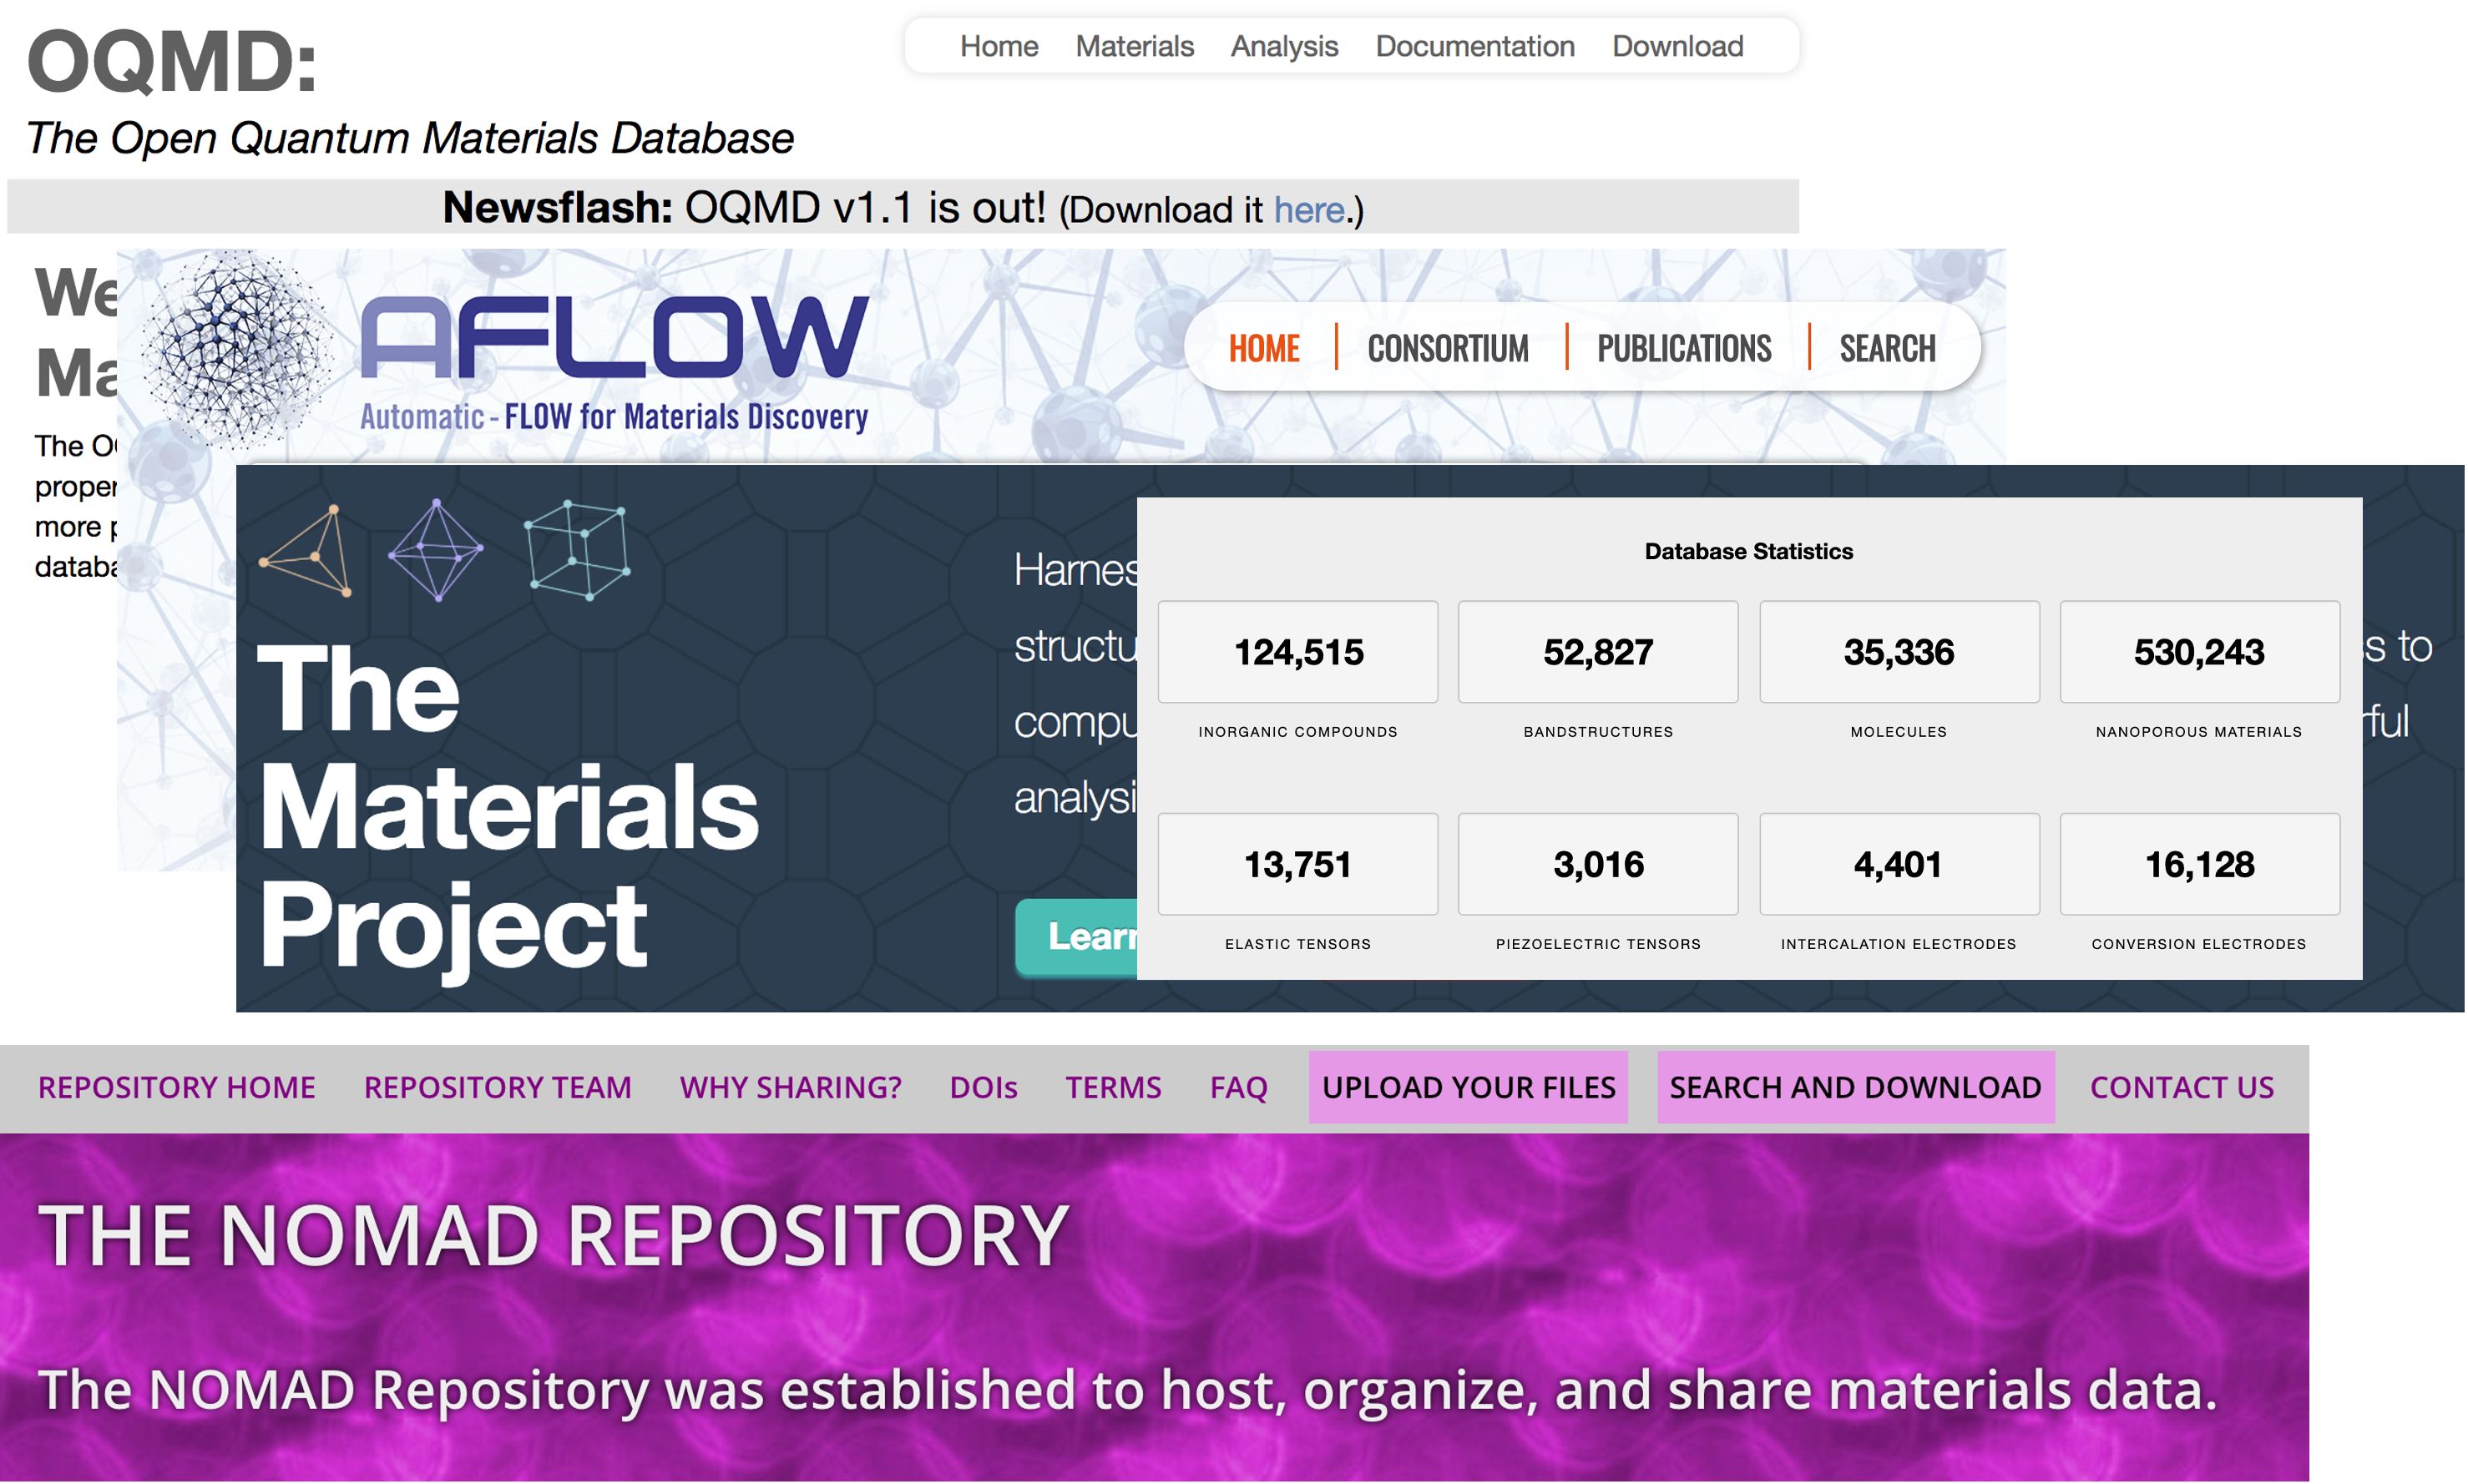
\includegraphics[width=0.7\textwidth]{lectures/slides_tex/materials_databases.png}
\end{figure}
\end{frame}


\begin{frame}{Google for Materials}
\begin{figure}
    \centering
    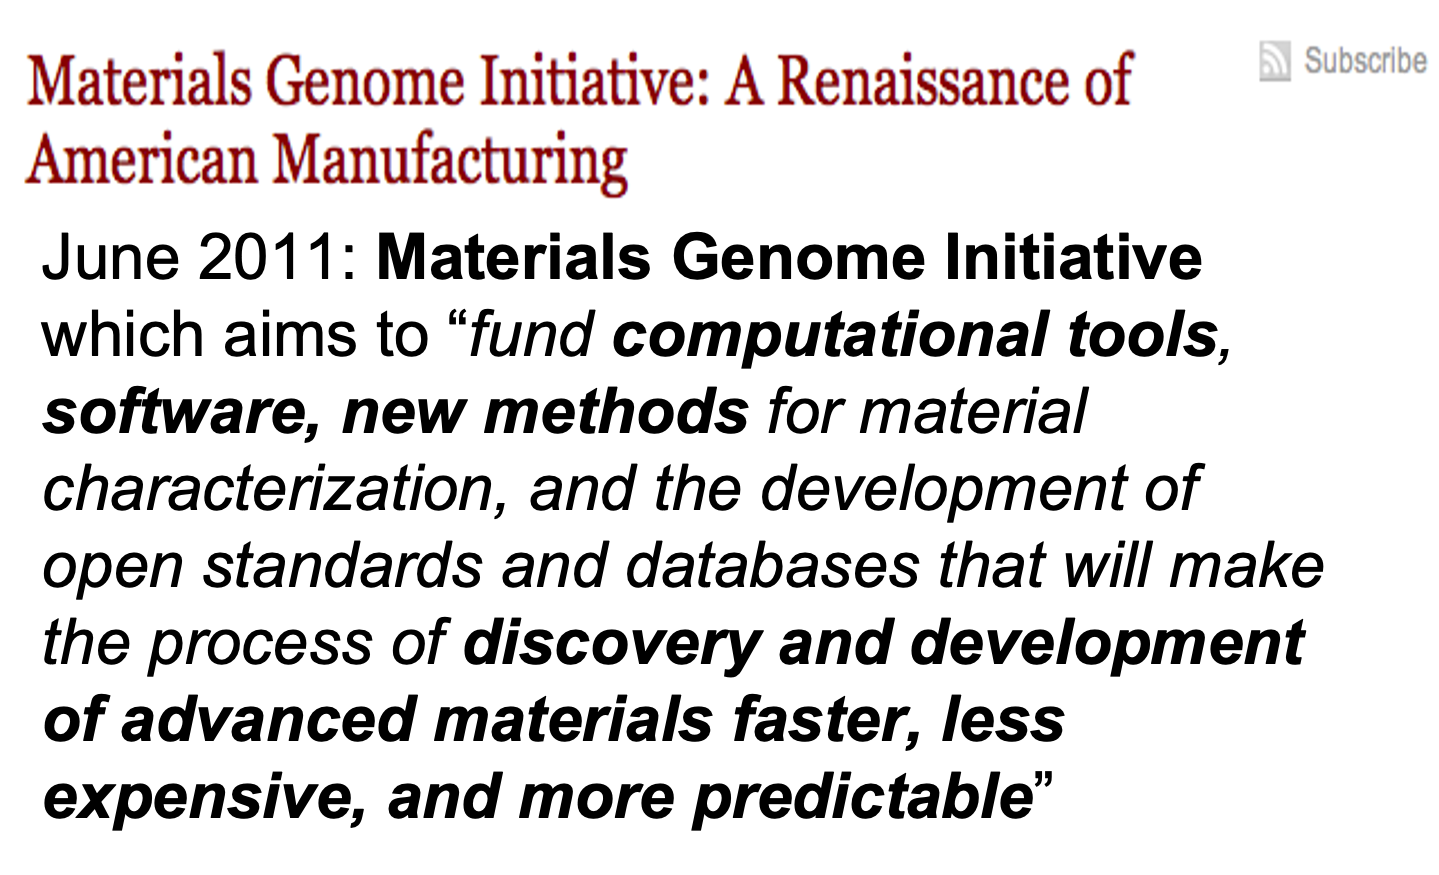
\includegraphics[width=0.45\textwidth]{lectures/slides_tex/mgi.png}
    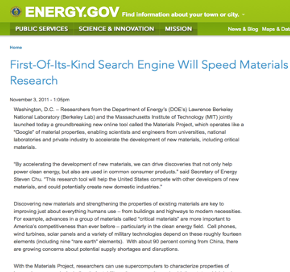
\includegraphics[width=0.25\textwidth]{lectures/slides_tex/doe_mp.png}
\end{figure}
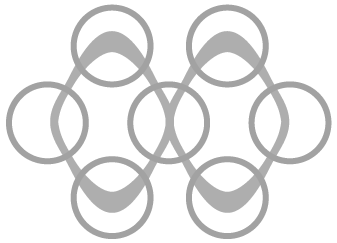
\includegraphics[width=0.1\textwidth]{lectures/slides_tex/mp_logo.png}
The Materials Project is an open science project to make the computed properties of all known inorganic materials publicly available to all researchers to accelerate materials innovation. 
\end{frame}


\begin{frame}{Google for Materials}
\begin{figure}
    \centering
    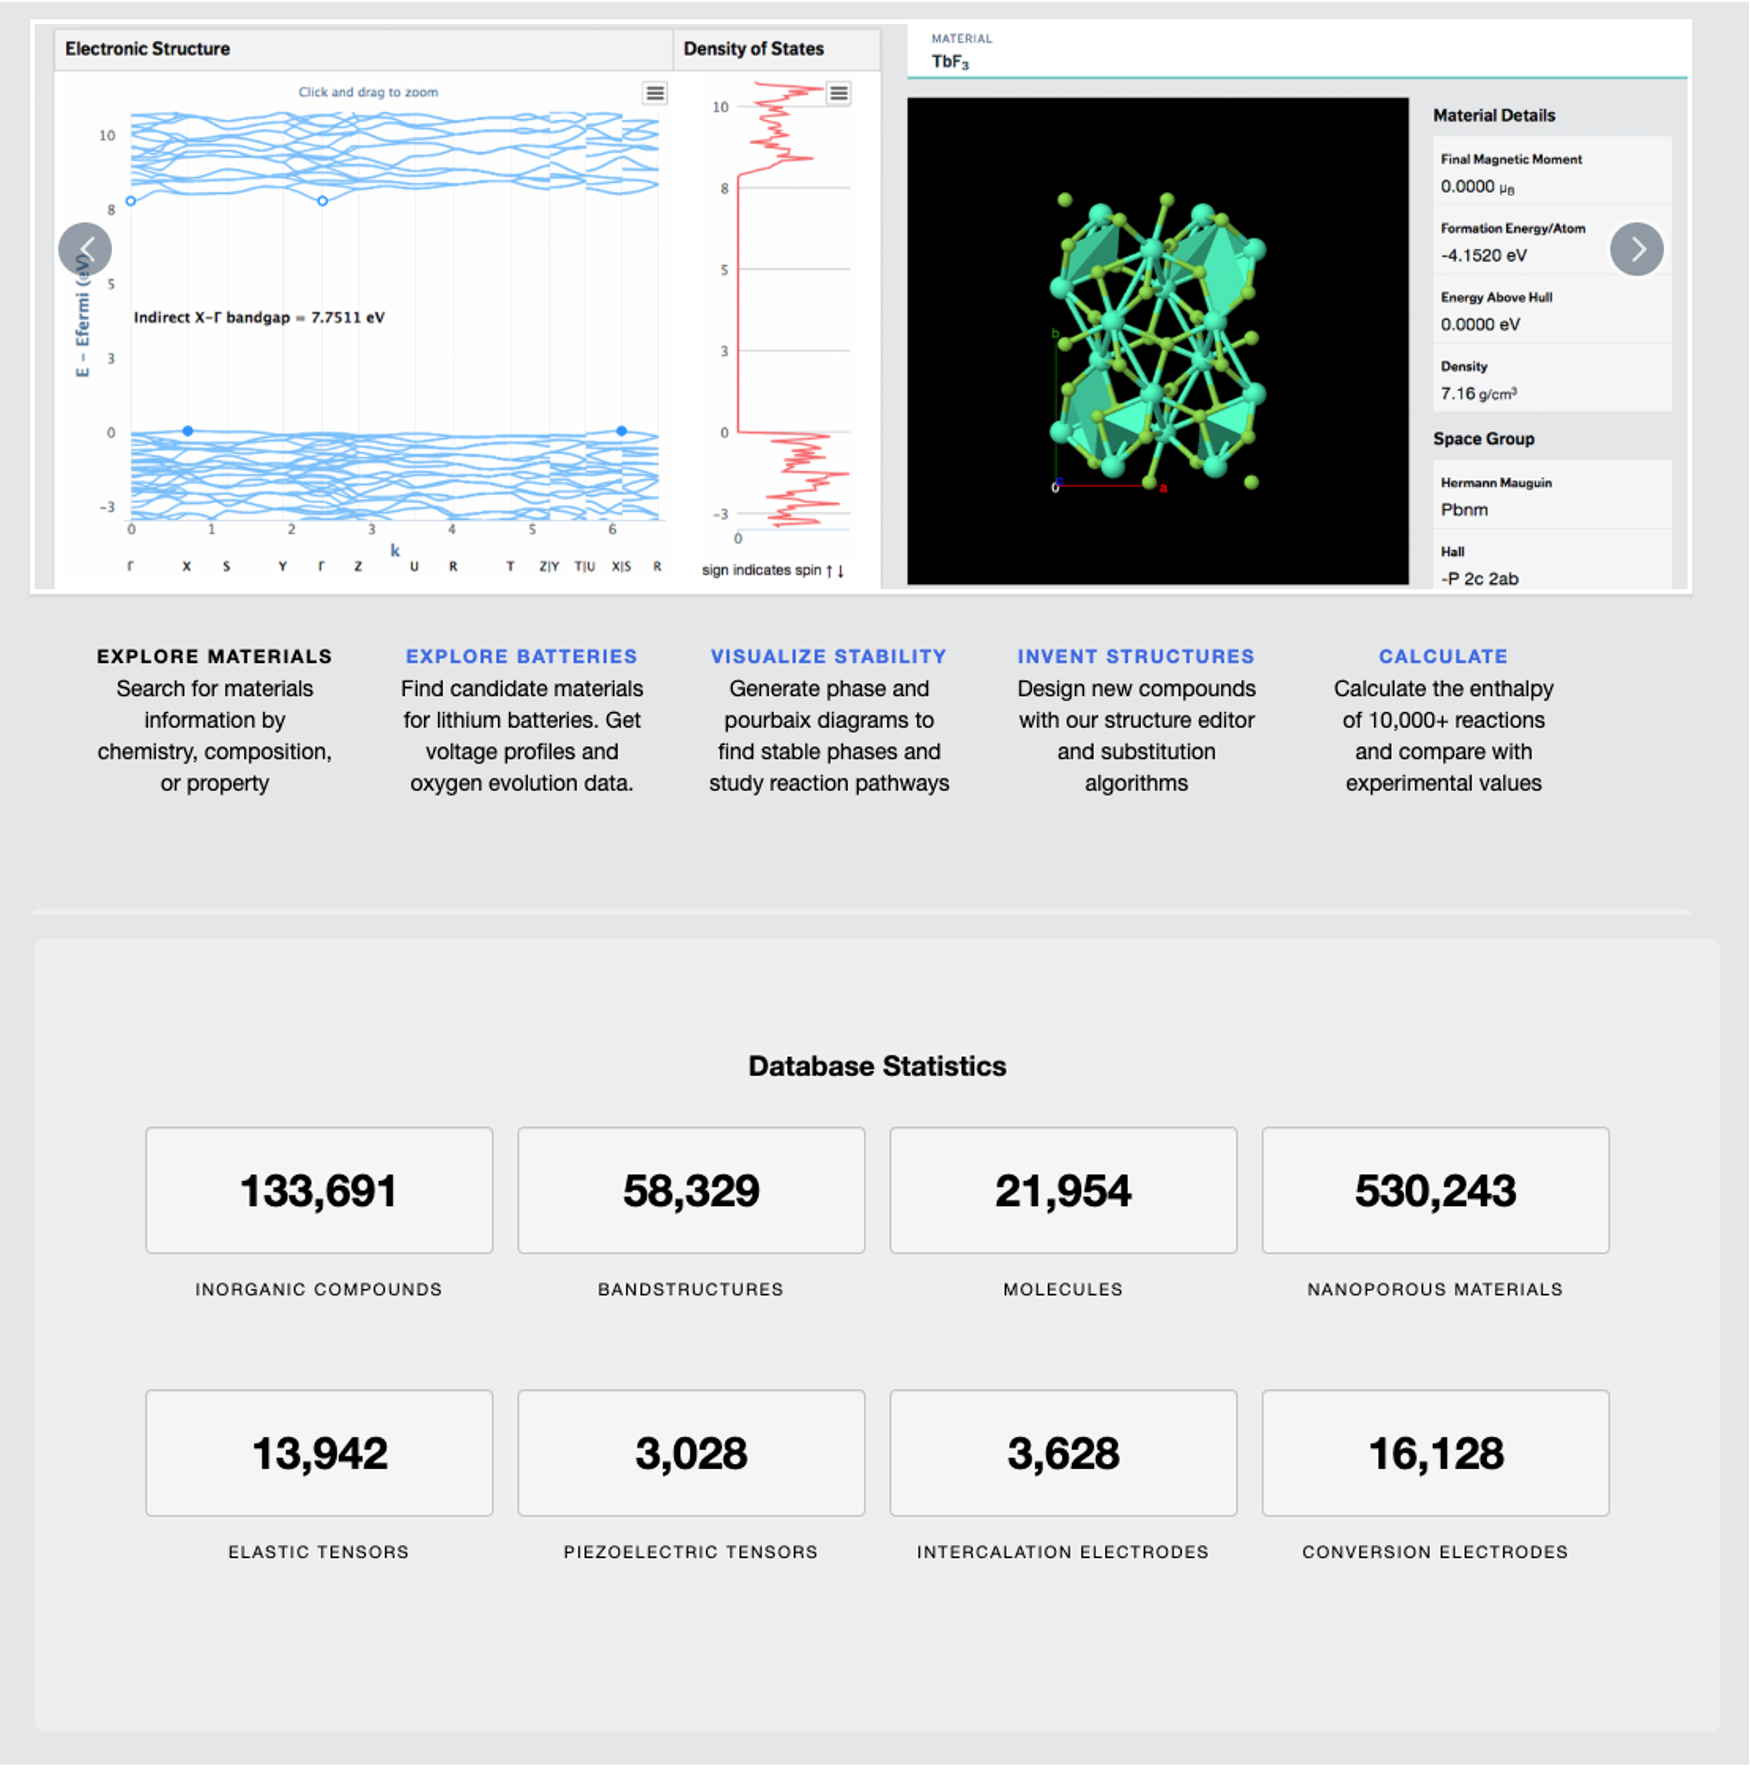
\includegraphics[width=0.40\textwidth]{lectures/slides_tex/mp_image1.png}
    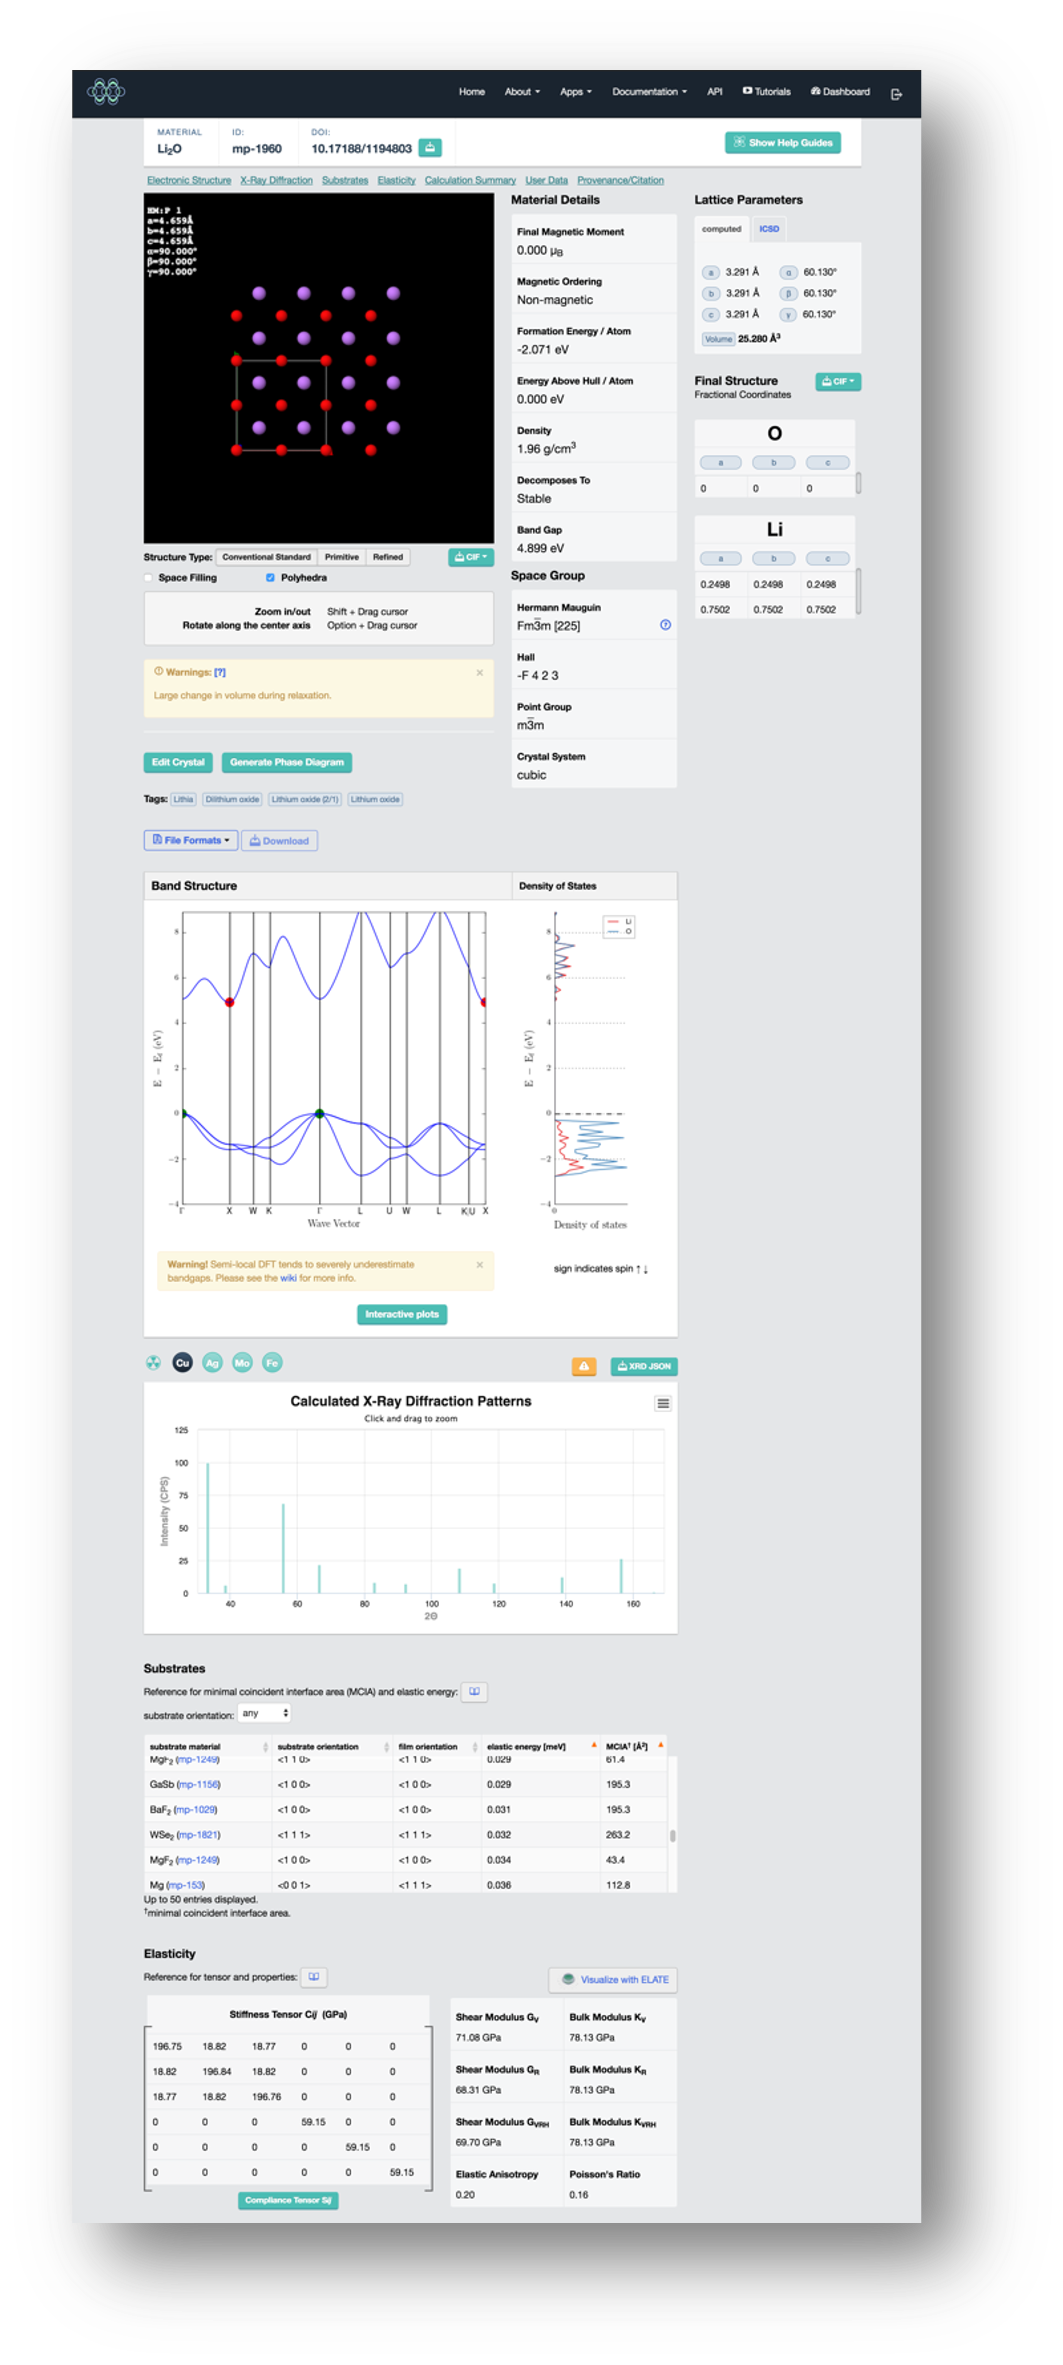
\includegraphics[width=0.20\textwidth]{lectures/slides_tex/mp_image2.png}
\end{figure}
\end{frame}


\begin{frame}{Materials API}
\begin{itemize}
    \item An open platform for accessing Materials Project data based on REpresentational State Transfer (REST) principles.
    \item \textit{Flexible and scalable} to cater to large number of users, with different access privileges.
    \item Simple to use and code agnostic.
\end{itemize}
\end{frame}


\begin{frame}[allowframebreaks]{Bibliography}
    \bibliographystyle{unsrt}
    \bibliography{refs}
\end{frame}


\begin{frame}
    \Huge{\centerline{The End}}
\end{frame}

\end{document}

